\documentclass[10pt]{standalone}
\input{../../tikzpic_packages.tex}

\begin{document}
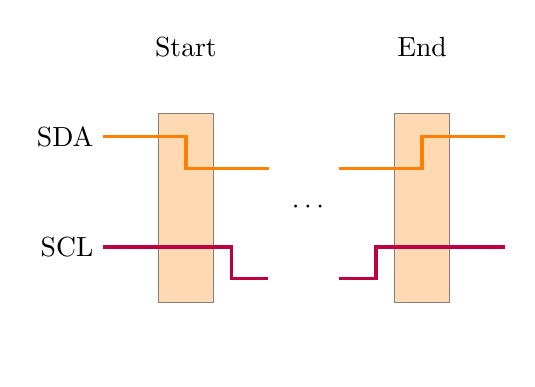
\begin{tikzpicture}[
scale = 1,
arrow/.style={-latex},
sda/.style={orange, very thick},
scl/.style={purple, very thick},
note/.style={help lines},
master/.style={fill=orange!30},
slave/.style={fill=blue!30}
]

\def\sdah{2.4}
\def\sdal{2}
\pgfmathsetmacro{\sdastep}{\sdah-\sdal}
\def\sclh{1}
\def\scll{.6}
\pgfmathsetmacro{\sclstep}{\sclh-\scll}


\def\frameb{.3}
\def\step{.7}
\pgfmathsetmacro{\steph}{\step*.5}
\pgfmathsetmacro{\stepd}{\step*.333}
%% Functions
\newcommand{\startseq}[1]{
\draw[note, master] (#1+\step,\sdah+\frameb)rectangle(#1+\step+\step,\scll-\frameb);
\draw[sda] (#1,\sdah)--++(\step,0)--++(\steph,0)--++(0,-\sdastep)--++(\steph,0)--++(\step,0);
\draw[scl] (#1,\sclh)--++(\step,0)--++(\step,0)--++(\stepd,0)--++(0,-\sclstep)--++(\stepd,0)--++(\stepd,0);
\path (#1+\step+\steph,\sdah+\frameb+.6)node[above]{Start};
}
\newcommand{\finalseq}[1]{
\draw[note, master] (#1+\step,\sdah+\frameb)rectangle(#1+\step+\step,\scll-\frameb);
\draw[sda] (#1,\sdal)--++(\step,0)--++(\steph,0)--++(0,\sdastep)--++(\steph,0)--++(\step,0);
\draw[scl] (#1,\scll)--++(\stepd,0)--++(\stepd,0)--++(0,\sclstep)--++(\stepd,0)--++(\step,0)--++(\step,0);
\path (#1+\step+\steph,\sdah+\frameb+.6)node[above]{End};
}

\path (0,\sdah)node[left]{SDA};
\path (0,\sclh)node[left]{SCL};


\startseq{0}
\path (2.6,1.5)node{$\cdots$};
\finalseq{3}

%% for same height as read & write:
\path[] (0,\scll-\frameb-.6)node{}--++(1,0);

\end{tikzpicture}
\end{document}